\section{Gaussian Process$^\ddagger$}
We denote the multivariate normal distribution as 
\begin{align}
    \Ng(\xv;\muv, \Sigma) \equiv \dfrac{1}{\sqrt{(2 \pi)^{N} |\Sigma|}} e^{- (\xv - \muv)^\top \Sigma^{-1}(\xv - \muv) /2  }.
\end{align}
When there is no risk of misunderstanding, we may also abbreviate the variable $\xv$ and write it as
\begin{align}
    \Ng(\muv, \Sigma) \equiv \dfrac{1}{\sqrt{(2 \pi)^{N} |\Sigma|}} e^{- (\xv - \muv)^\top \Sigma^{-1}(\xv - \muv) /2  }
\end{align}

\subsection*{Gaussian Process as a Correlated Noise}

A Gaussian process is a stochastic process of a random variable $\xv$ that follows a multivariate normal distribution
\begin{align}
\dv \sim \Ng(\zerov,\Sigma)
\end{align}
Suppose $d_i$ represents a time series; if each component of the covariance matrix of this multivariate normal distribution is given as
\begin{align}
\Sigma_{ij} = K_{ij}(a, \tau) = a k(|t_i-t_j|; \tau),
\end{align}
namely as a function of the absolute difference between $t_i$ and $t_j$, then we obtain a Gaussian process with correlation length $\tau$.
Various types of kernel functions $k(t,\tau)$ are possible. For example, the RBF kernel
\begin{align}
 k_\mathrm{RBF}(t;\tau) = \exp{\left(- \frac{t^2}{2 \tau^2} \right)},
\end{align}
and the Mat\'{e}rn 3/2 kernel
\begin{align}
\label{eq:MaternA}
 k_\mathrm{M3/2}(t;\tau) = \left( 1 + \frac{\sqrt{3} t}{\tau} \right) e^{- \sqrt{3} t/\tau}. 
\end{align}
are common choices.

If we sample data points from such a Gaussian process, the result looks like Fig.~\ref{fig:gp1}. Here, additional Gaussian noise with zero mean and standard deviation $\sigma$ has been added to the data. For convenience, let us call this noise the observational noise.
\begin{figure}[htb]
\begin{center}
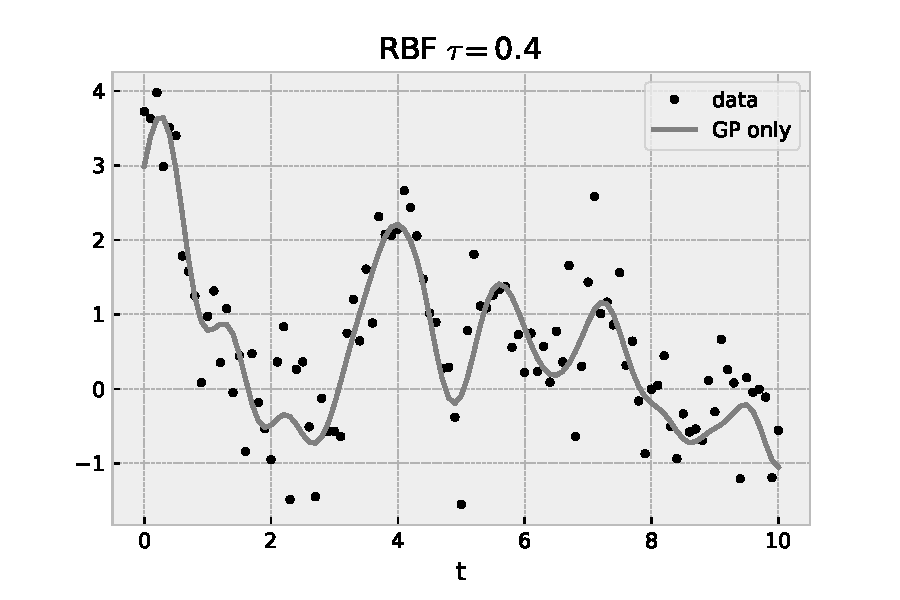
\includegraphics[width=\linewidth]{fig/gp/gp1.pdf}
\caption{Data sampled from a Gaussian process. The solid line shows the case without observational noise of amplitude $\sigma$.\label{fig:gp1}}
\end{center}
\end{figure}

Now, let us attempt MCMC sampling of $\tau$, $a$, and $\sigma$ based on these data. Since Gaussian observational noise with zero mean and standard deviation $\sigma$ was added, the probabilistic model is
\begin{eqnarray}
\label{eq:gpmodel0}
\dv &\sim& \Ng(\zerov,\Sigma^\prime ) \\
\Sigma^\prime &=& K(a, \tau) + \sigma^2 I
\end{eqnarray}
Here, $\Sigma^\prime$ assumes the RBF kernel with an additional diagonal term representing independent errors. That is,
\begin{align}
 \Sigma_{ij} (a, \tau, \sigma) = a k_\mathrm{RBF} (|t_i - t_j|; \tau) + \sigma^2 I
\end{align}
so that the covariance depends on the parameters $(a, \tau, \sigma)$. By using the exponential distribution $E(x)$ to define the priors, for example, the prior distributions are
\begin{align}
    p(a) &= E(1) \\
    p(\tau) &= E(1) \\
    p(\sigma) &= E(1) 
\end{align}
and the likelihood is written as
\begin{align}
    p(\dv|a, \tau, \sigma) = \Ng(\dv;\zerov,  \Sigma (a, \tau, \sigma) ).
\end{align}
Thus, we can perform MCMC sampling.

The posterior distribution sampled using HMC is visualized in Fig.~\ref{fig:gp2}.
\begin{figure}[htb]
\begin{center}
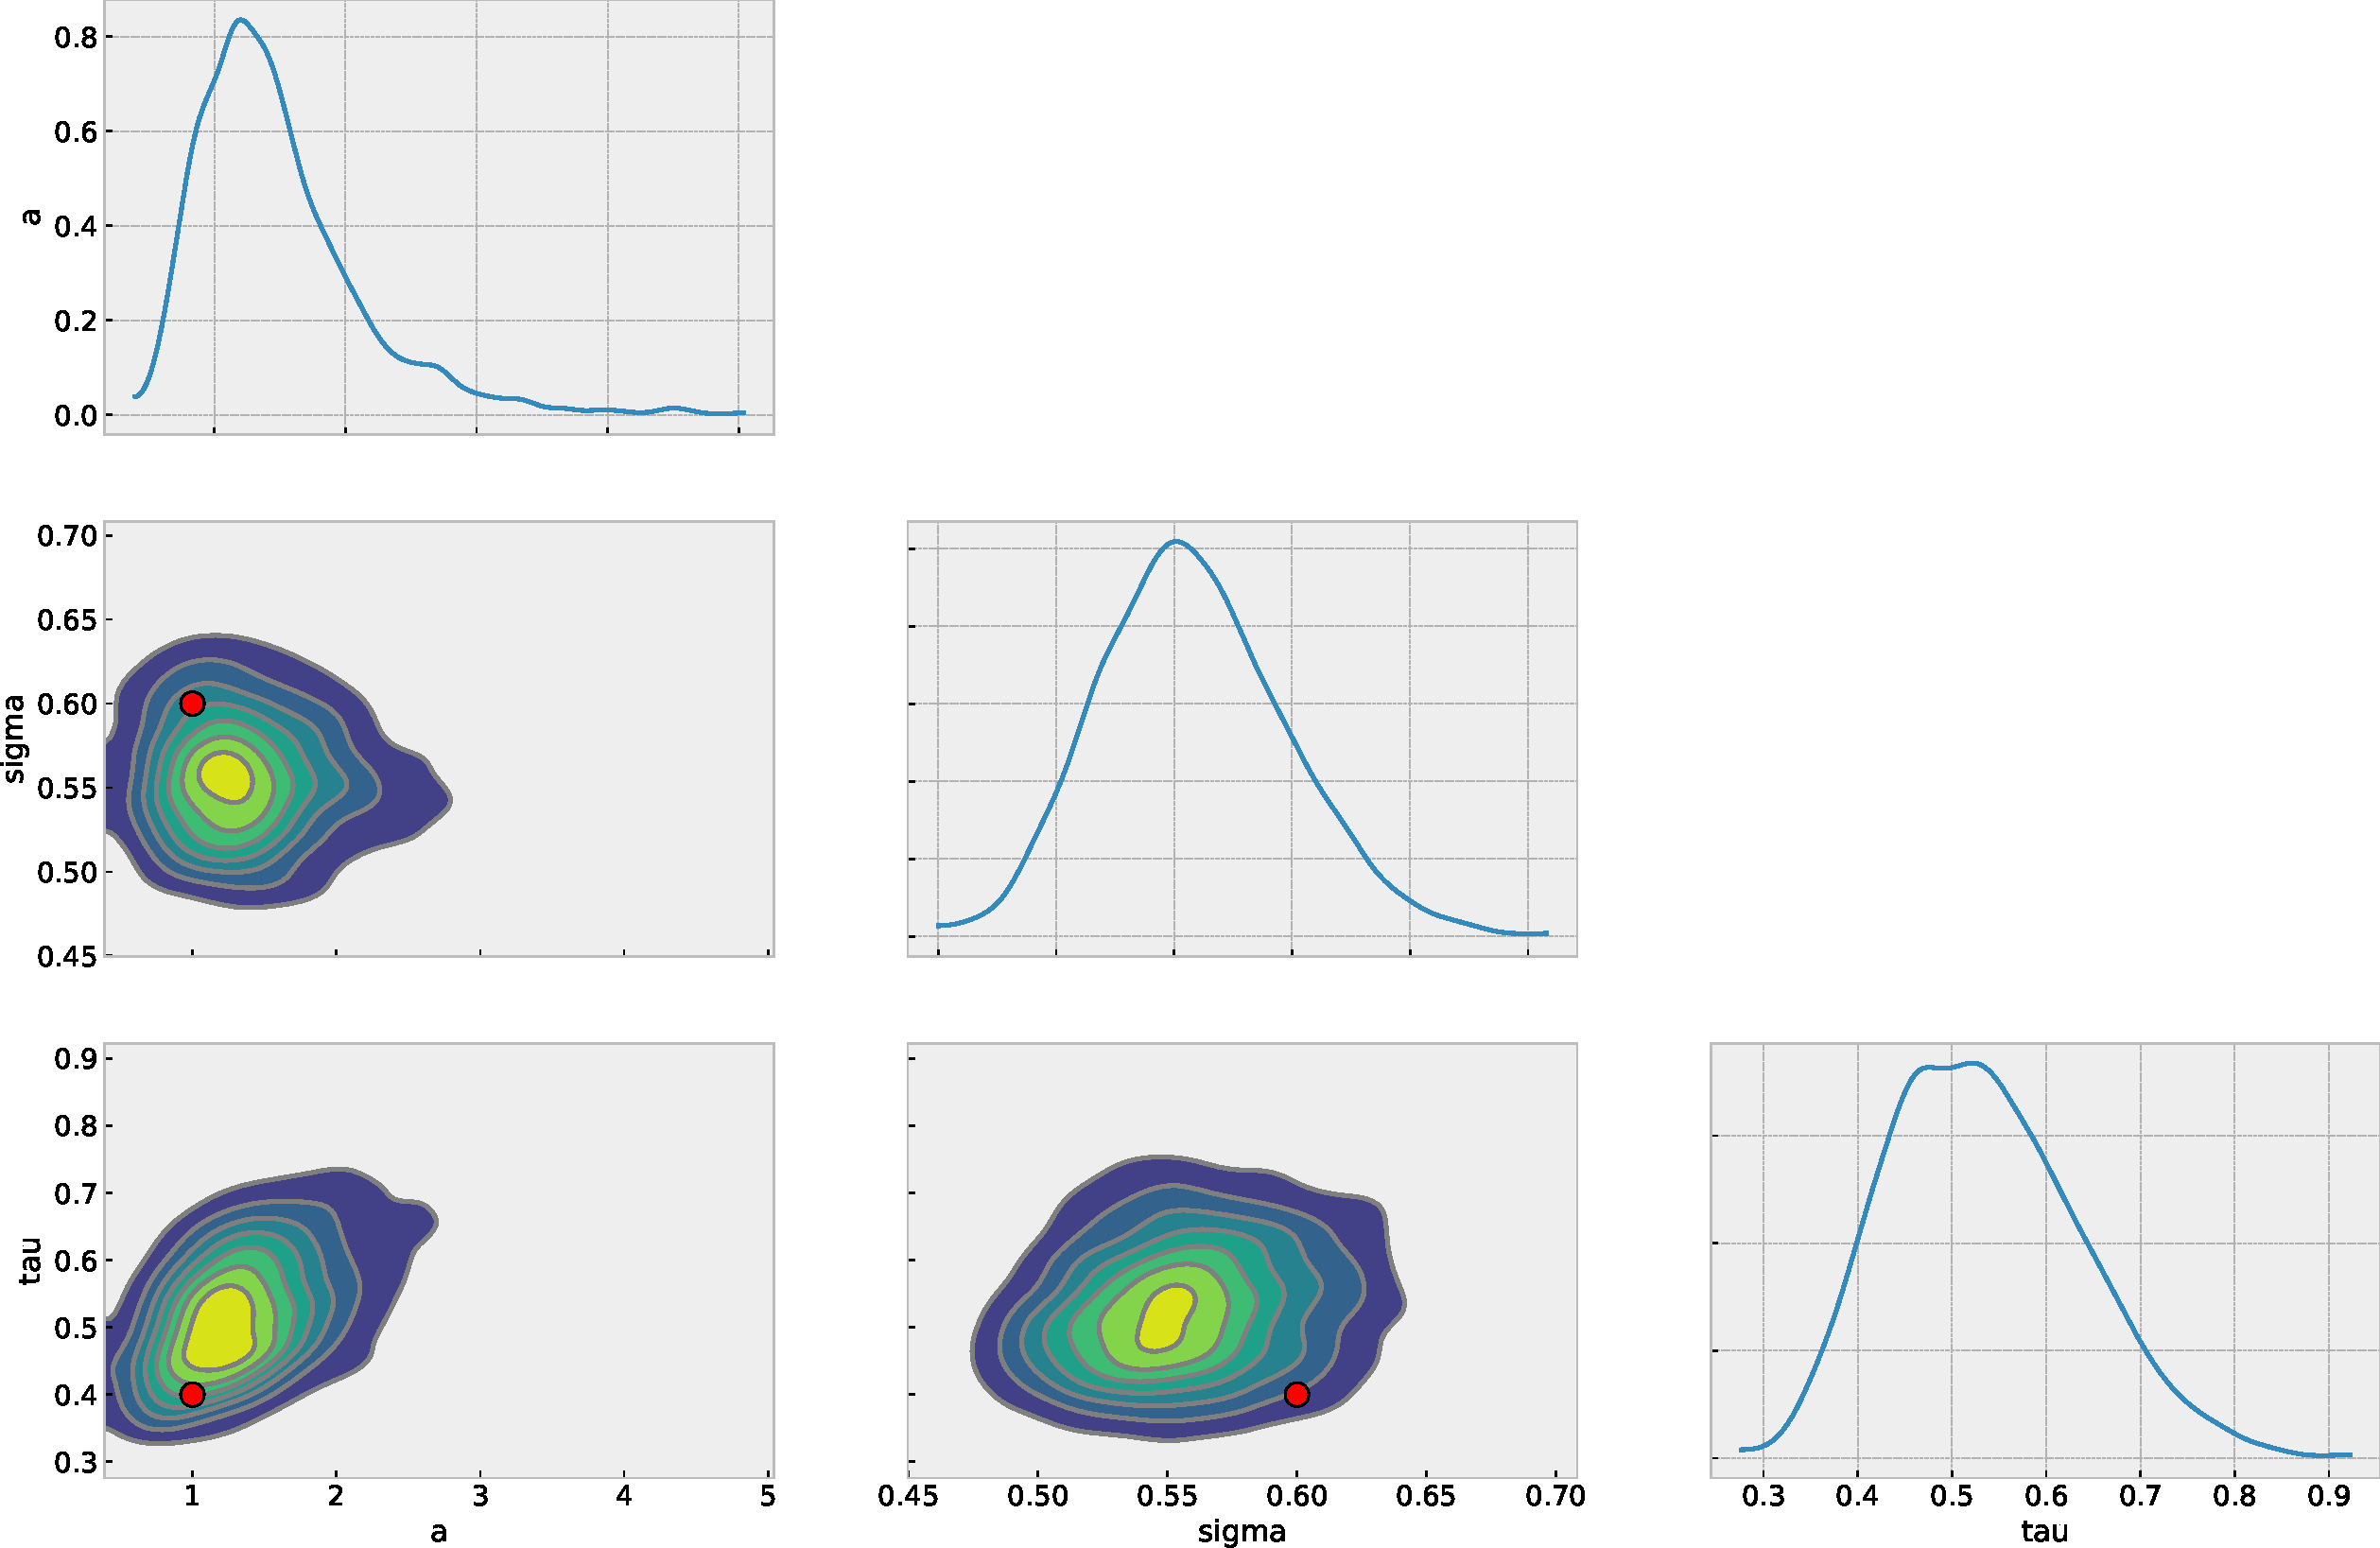
\includegraphics[width=\linewidth]{fig/gp/gp2.pdf}
\caption{\label{fig:gp2}}
\end{center}
\end{figure}
In the modeling viewpoint of Eq.~(\ref{eq:gpmodel0}), the model mean is $\xv=\zerov$. This is intuitively seen in the credible interval shown in Fig.~\ref{fig:gp3}.
\begin{figure}[htb]
\begin{center}
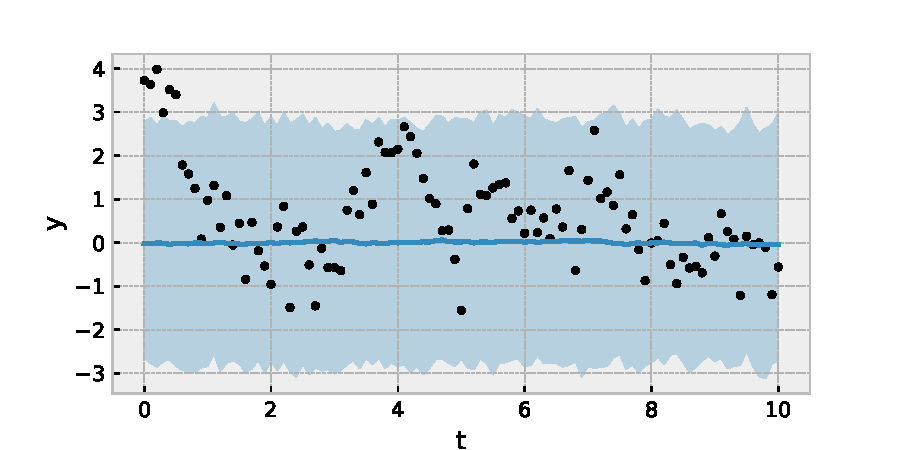
\includegraphics[width=\linewidth]{fig/gp/gp3.pdf}
\caption{\label{fig:gp3}}
\end{center}
\end{figure}

\subsection*{Gaussian Process as a Prior Distribution for Model Parameters}

The Gaussian process analysis described above can also be viewed as setting the prior distribution for the model parameters $\mv$ as
\begin{align}
p(\mv) = \Ng (\mv; \zerov,\Sigma),
\end{align}
and regarding the data as
\begin{align}
d_i &= m_i + \epsilon \\
\epsilon &\sim \Ng (0,\sigma^2),
\end{align}
where $\epsilon$ corresponds to observational noise. More explicitly, if we write the model $\gv$ as the identity transformation, then
\begin{align}
\label{eq:identif}
\gv(\mv) &= \mv \\
\dv &= \gv(\mv) + \epsilonv \\
\epsilonv &\sim \Ng (\boldsymbol{0} ,\sigma^2 I),
\end{align}
so that the likelihood function becomes
\begin{align}
p(\dv|\mv) &= \Ng (\dv ; \gv(\mv),  \boldsymbol{0} ,\sigma^2 I) = \Ng (\dv ; \mv,\sigma^2 I).
\end{align}
Moreover, the prior distribution itself contains parameters, i.e.,
\begin{align}
\Sigma_{ij} = a k(|t_i-t_j|;\tau),
\end{align}
where the parameters $a$ and $\tau$ are referred to as hyperparameters. Assuming prior distributions for these hyperparameters (often called hyperpriors) is then required.

When the hyperparameters are fixed, it is known that the posterior distribution of $\mv$ can be written analytically. Here, let us outline the Gaussian process calculation. Since the product of two multivariate normal distributions is again a multivariate normal distribution, it suffices to compute only the exponent part of the Gaussian. The exponent part of the multivariate normal distribution is
\begin{align}
\label{eq:gp}
&- 2 \log{ \Ng(\mv; \muv, \Sigma) } = (\mv - \muv)^\top \Sigma^{-1} (\mv - \muv) \nonumber \\
&= \mv^\top \Sigma^{-1} \mv - 2 \mv^T \Sigma^{-1} \muv + \mathrm{const}.
\end{align}
Thus, if a probability density $p(\mv)$ known to follow some multivariate normal distribution can be written as
\begin{align}
\label{eq:gpqu}
- 2 \log{ p(\mv) } = \mv^\top P \mv - 2 \mv^\top \qv + \mathrm{const},
\end{align}
then, by comparison with Eq.~(\ref{eq:gp}), this density must be
\begin{align}
\label{eq:gpqusol}
p(\mv) = \Ng(\mv; P^{-1} \qv ,P^{-1}).
\end{align}

Now, since the posterior distribution is
\begin{align}
\label{eq:gppos}
p(\mv|\dv) \propto p(\dv|\mv) p(\mv) = \Ng (\dv ; \mv,\sigma^2 I) \Ng (\mv;\zerov,\Sigma),
\end{align}
expanding the exponent part with respect to $\mv$ yields
\begin{align}
\label{eq:gpposs}
&- 2 \log{[\Ng (\dv;\mv,\sigma^2 I) \Ng (\mv;\zerov,\Sigma)]} \nonumber \\
&= \mv^\top (\Sigma^{-1} + \sigma^{-2} I ) \mv - 2 \sigma^{-2} \mv^\top \dv + \mathrm{const}.
\end{align}
Furthermore, using
\begin{align}
\label{eq:gppossxx}
(\Sigma^{-1} + \sigma^{-2} I )^{-1} = \Sigma (I + \sigma^{-2} \Sigma )^{-1},
\end{align}
we obtain
\begin{align}
\label{eq:gpposss}
p(\mv|\dv) = \Ng (\mv;\Sigma (\sigma^{2} I + \Sigma )^{-1} \dv, \Sigma (I + \sigma^{-2} \Sigma )^{-1} ).
\end{align}

By MCMC we can sample $\tau$ and $\sigma$, but let us consider what the posterior distributions of these parameters mean. Within the current framework, these can be regarded as hyperparameters, so we define $\thetav = (a, \tau, \sigma)^\top$ as the vector of hyperparameters. From here on, we will treat $\thetav$ probabilistically as well. Now, the marginalized likelihood over $\mv$ is
\begin{align}
\label{eq:gppozz}
p(\dv|\thetav) = \frac{p(\dv|\mv,\thetav) p(\mv,\thetav)}{p(\mv|\dv,\thetav)},
\end{align}
which is still a multivariate normal distribution. Considering only the terms involving $\dv$ in the exponent part, we obtain
\begin{align}
\label{eq:gppozzp}
&- 2 \log p(\dv|\thetav) = \nonumber \\
&- 2 \log p(\dv|\mv,\thetav) + 2 \log p(\mv|\dv,\thetav) + \mathrm{const} \nonumber \\
&= - 2 \log \Ng(\dv; \mv, \sigma^2 I )  \nonumber \\
&+ 2 \log \Ng(\mv;\Sigma (\sigma^{2} I + \Sigma )^{-1} \dv, \Sigma (I + \sigma^{-2} \Sigma )^{-1} ) \nonumber \\
&= \dv^\top (\sigma^{2} I + \Sigma)^{-1} \dv + \mathrm{const.}
\end{align}
Therefore,
\begin{align}
\label{eq:gmarg}
p(\dv|\thetav) =  \Ng (\dv;\zerov, \Sigma + \sigma^{2} I ).
\end{align}
\underline{If $\Sigma = K(\tau)$, this is equivalent to Eq.~(\ref{eq:gpmodel0}).}  
That is, given a (hyper)prior distribution $p(\thetav)$, the marginalized posterior distribution is
\begin{align}
\label{eq:gmpost}
p(\thetav|\dv) \propto p(\dv|\thetav) p(\thetav),
\end{align}
which is what we are sampling.

Figure~\ref{fig:gp2} can therefore be understood as showing the marginalized posterior distribution of the hyperparameters $\tau$ and $\sigma$. In other words, for $k=0,..., N_s-1$,
\begin{align}
\label{eq:gmposts}
\thetav^\dagger_k \sim p(\thetav|\dv) \propto p(\dv|\thetav) p(\thetav),
\end{align}
we have sampled these. Using these samples together with Eq.~(\ref{eq:gpposss}), and noting that
\begin{align}
\label{eq:gpposssaq}
p(\mv, \thetav|\dv) = p(\mv|\thetav, \dv) p(\thetav|\dv),
\end{align}
it follows that
\begin{align}
\label{eq:gpposssaahuq}
 p(\mv|\thetav^\dagger_k, \dv) &= \Ng ( \muv_k ,  K_k ), \\
 \label{eq:muvk}
 \muv_k &= K(a^\dagger_k,\tau^\dagger_k) ((\sigma^\dagger_k)^{2} I + K(a^\dagger_k,\tau^\dagger_k) )^{-1} \dv, \\
  \label{eq:Kk}
 K_k &= K(a^\dagger_k,\tau^\dagger_k)(I + (\sigma^\dagger_k)^{-2} K(a^\dagger_k,\tau^\dagger_k) )^{-1},
\end{align}
so that the sampled sets $(\mv^\dagger_k,\thetav^\dagger_k)$ satisfy
\begin{align}
\label{eq:gpposssaqp}
(\mv^\dagger_k,\thetav^\dagger_k) \sim p(\mv, \thetav|\dv).
\end{align}
\footnote{While there is abundant literature on methods using point estimates of hyperparameters (so-called maximum marginal likelihood or maximum evidence), discussions of resampling from the marginalized posterior are harder to find. For reference, the author has previously discussed this in the context of Bayesian linear problems with Gaussian processes \cite{2020ApJ...900...48K}.}

By computing the HPDI, we obtain the credible interval for $\mv$ shown in Fig.~\ref{fig:gp4}. It should be noted that this represents the 90\% interval of the model $\mv$, and not the prediction of $\dv$ including observational noise.
\begin{figure}[htb]
\begin{center}
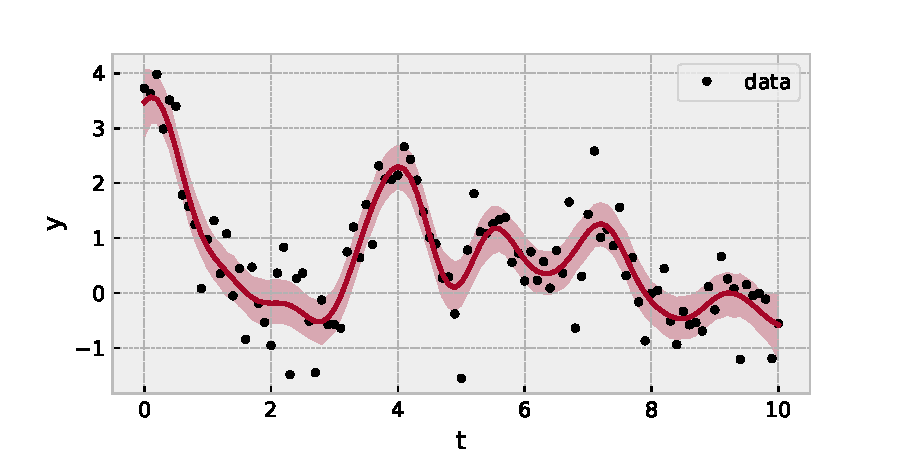
\includegraphics[width=\linewidth]{fig/gp/gp4.pdf}
\caption{\label{fig:gp4}}
\end{center}
\end{figure}
\subsection*{Prediction at Locations Without Data Points}

Now, in general, what is the predictive value at $t=t^\ast$? In what follows, we omit the hyperparameters for simplicity of notation. First, when $\mv$ and $\mva$ follow a Gaussian process,
\begin{align}
p(\mva|\mv) = \Ng (K_{\times}^\top K^{-1}  \mv, K_\ast - K_\times^\top K^{-1} K_\times),
\end{align}
where
\begin{align}
K_{ij} &= a k(|t_i-t_j|;\tau), \\
(K_{\times})_{ij} &= a k(|t_i-t^\ast_j|;\tau), \\
(K_{\ast})_{ij} &= a k(|t^\ast_i-t^\ast_j|;\tau).
\end{align}

Similarly,
\begin{align}
\label{eq:predgp1}
p(\mva|\dv) =  \Ng (K_{\times}^\top K_\sigma^{-1}  \dv, K_{\ast} - K_\times^\top K_\sigma^{-1} K_\times),
\end{align}
where
\begin{align}
(K_{\sigma})_{ij} = a k(|t_i-t_j|;\tau) + \sigma^2 \delta_{i,j},
\end{align}
and $\delta_{i,j}$ is the Kronecker delta. Here, $p(\mva|\dv)$ is the posterior distribution of the Gaussian process regarded as the model parameters, and thus observational noise is not taken into account.

If we wish to make predictions including observational noise, then, based on the model
\begin{align}
\dv^\ast = \mv^\ast + \epsilonv,
\end{align}
we obtain
\begin{align}
\label{eq:predgp2}
p(\dv^\ast|\dv) =  \Ng (K_{\times}^\top K_\sigma^{-1} \dv, K_{\ast,\sigma} - K_\times^\top K_\sigma^{-1} K_\times),
\end{align}
where
\begin{align}
(K_{\ast,\sigma})_{ij} &= a k(|t^\ast_i-t^\ast_j|;\tau) + \sigma^2 \delta_{i,j}.
\end{align}

Thus, by performing sampling including the hyperparameters, one can evaluate Eqs.~(\ref{eq:predgp1}, \ref{eq:predgp2}) and compute the credible intervals. Figure~\ref{fig:gp6} shows the HPDI results. The darker region corresponds to the credible interval of $\mva$, while the lighter region corresponds to that of $\dv^\ast$.

\begin{figure}[htb]
\begin{center}
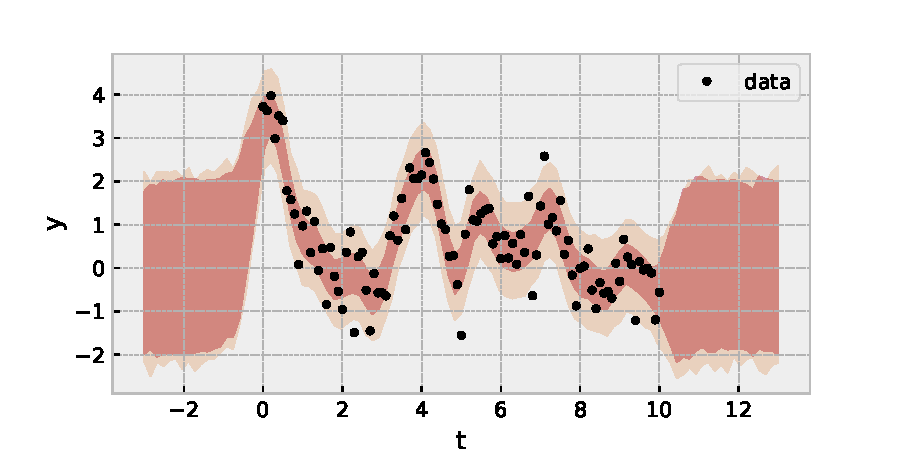
\includegraphics[width=\linewidth]{fig/gp/gp6.pdf}
\caption{\label{fig:gp6}}
\end{center}
\end{figure}


\section{Gaussian Process as a Model$^\ddagger$}

So far, we have considered as a model a Gaussian process with zero mean generating the data:
\begin{align}
\mv \sim \Ng ({\bf 0},\Sigma(\tv)).
\end{align}
Here, we instead consider the case in which the data are generated by a Gaussian process whose mean is a function of $t$, namely
\begin{align}
\label{eq:modelgp}
\mv \sim \Ng (\fv(\tv),\Sigma(\tv)),
\end{align}
where $\fv(\tv)$ is the vector obtained by applying $f(t)$ element-wise to $\tv=(t_0,t_1,\cdots t_{N-1})$. In this case, let us consider the following functional form for $f(t)$:
\begin{align}
f(t) = k e^{-(t-T_0)^2/2 s^2} \sin{(2 \pi t/P)}.
\end{align}
Although we wrote $f(t)$ for simplicity above, we also denote it as $f(t;\thetav)$ when emphasizing the dependence on parameters $\thetav=(T_0,k,s,P)$.

If the covariance matrix in Eq.~(\ref{eq:modelgp}) is chosen to be an RBF kernel, then data such as those in the upper panel of Fig.~\ref{fig:gp1m} are generated. Here, $\tau=3$, and we can see that a relatively smooth trend is superimposed on $f(t)$.
\begin{figure}[htb]
\begin{center}
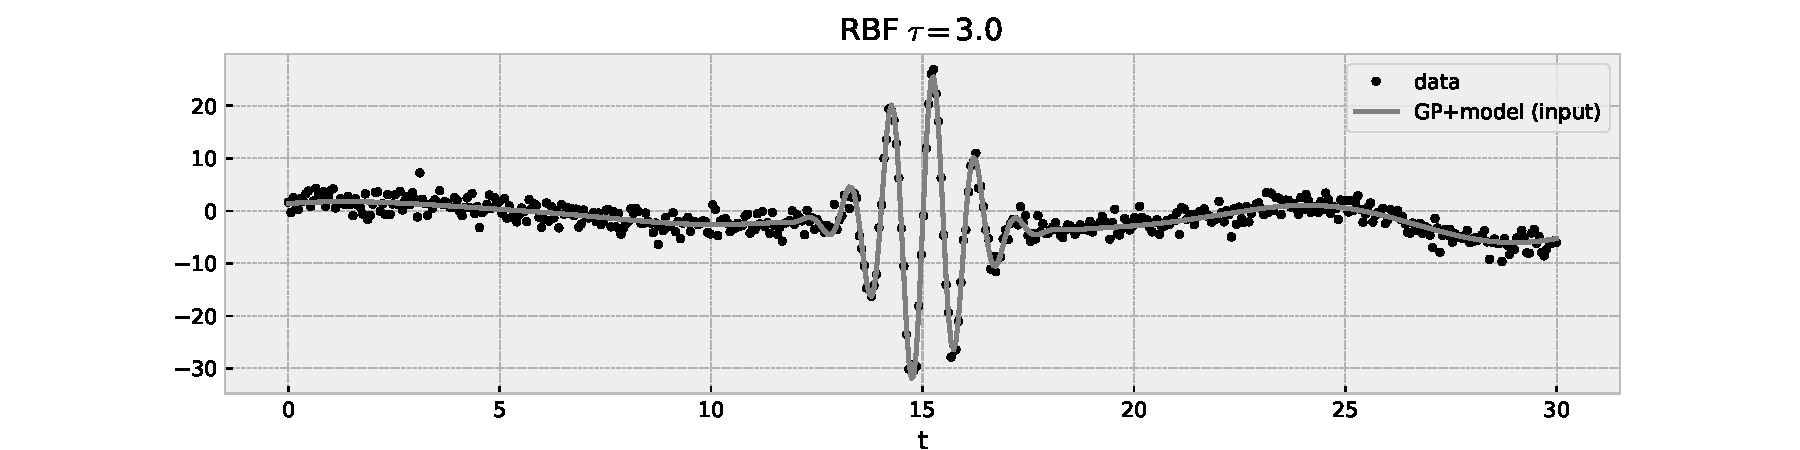
\includegraphics[width=\linewidth]{fig/gpmodel/gp1.pdf}
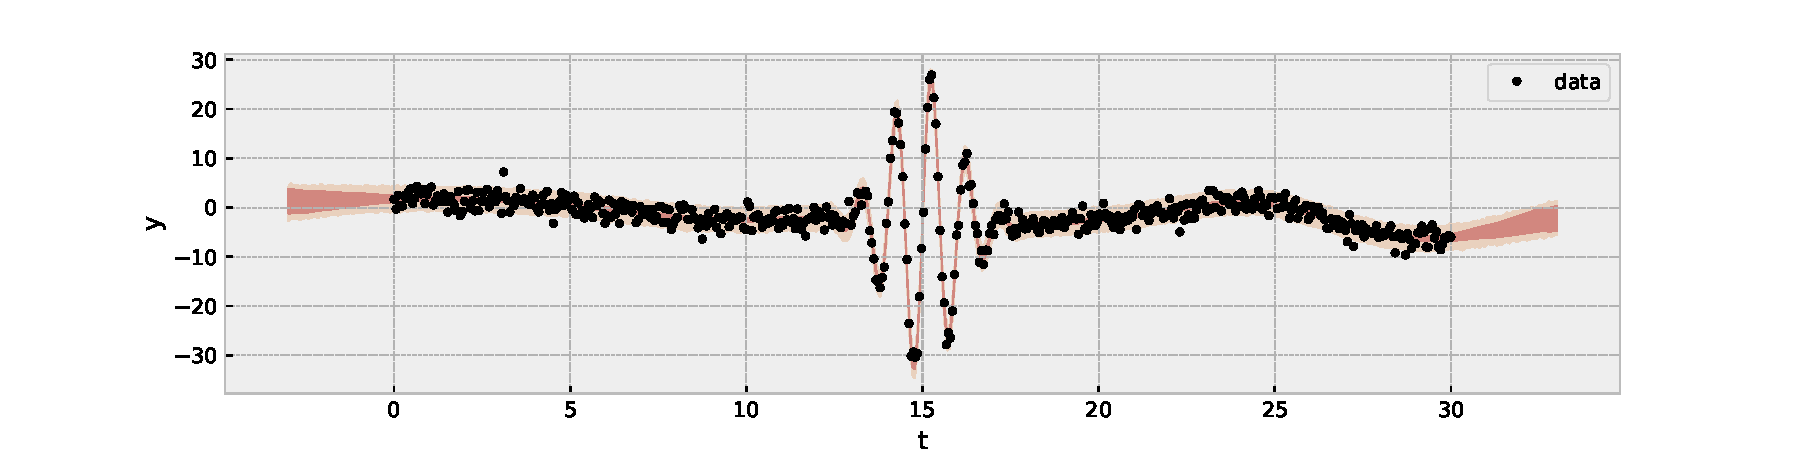
\includegraphics[width=\linewidth]{fig/gpmodel/gp6.pdf}
\caption{The solid line shows the case without observational noise of amplitude $\sigma$.\label{fig:gp1m}}
\end{center}
\end{figure}
Fitting such a model with HMC corresponds to modeling correlated noise plus observational noise along with the signal $f(t)$, in order to estimate the parameters of $f(t)$.

When $\fv(\tv)$ is known, the predictive distributions without and with observational noise are, respectively,
\begin{align}
\label{eq:predgp_model}
&p(\mva|\dv) =   \nonumber \\
&\Ng (\fv(\tv^\ast) + K_{\times}^\top K_\sigma^{-1}  (\dv - \fv(\tv)),  K_{\ast} - K_\times^\top K_\sigma^{-1} K_\times), \\
&p(\dv^\ast|\dv) =   \nonumber \\
&\Ng (\fv(\tv^\ast) + K_{\times}^\top K_\sigma^{-1} (\dv - \fv(\tv)), K_{\ast,\sigma} - K_\times^\top K_\sigma^{-1} K_\times).
\end{align}
Since the parameters $\thetav=(T_0,k,s,P)$ of $\fv(t)$ are sampled with HMC, for the latter case, for example, using each sampled $\thetav^\dagger_k$, one can sample
\begin{align}
\label{eq:predgp2_}
&\dv^\ast_k \sim  \Ng (\mu_k, K_k), \\
&\mu_k = \fv(\tv^\ast; \thetav^\dagger_k) + K_{\times}^\top K_\sigma^{-1} (\dv - \fv(\tv; \thetav^\dagger_k)), \\
&K_k = K_{\ast,\sigma} - K_\times^\top K_\sigma^{-1} K_\times,
\end{align}
thereby obtaining predictive samples. In this way, Gaussian process fitting can be performed including the model $f(t)$ itself, as shown in the lower panel of Fig.~\ref{fig:gp1m}.
